\documentclass[nobib]{MSword}
% Class options:
%-------------------------------
% nobib         - skip bibliography code/ don't include bib
% math          - include math packages and useful math commands
% hidelinks     - hide hyperref colored link boxes
% wordlinks     - link color scheme similar to word


% Preamble code:
%%%%%%%%%%%%%%%%%%%%%%%%%%%%%%%%%%%%%%%%
\usepackage[english]{babel}
\usepackage{csquotes}
\usepackage{lipsum}

% % Uncomment using "Ctrl + /" (/ on numpad):
% % Customizing headers and footers:
% \fancypagestyle{custom}{%
%     \fancyhf{}% clears the footer and header
%     % Header:
%     \fancyhead[L]{}
%     \fancyhead[C]{}
%     \fancyhead[R]{}
%     % Footer:
%     \fancyfoot[L]{}
%     \fancyfoot[C]{}
%     \fancyfoot[R]{}
%         % Tips:
%         % ----
%         % L: left, C: center, R: right
%         % O: odd pages, E: even pages
%         % ----
%         % Example: \fancyghead[LO,RE]{Text}
%         % will produce "Text" left in the header
%         % on odd pages and right in the header on even pages.
%     % Rules/ lines:
%     \renewcommand{\headrulewidth}{0.4pt}
%     \renewcommand{\footrulewidth}{2pt}
% }
% % Changing the pagestyle:
% \pagestyle{custom}

%%%%%%%%%%%%%%%%%%%%%%%%%%%%%%%%%%%%%%%%

% Preamble information:
%%%%%%%%%%%%%%%%%%%%%%%%%%%%%%%%%%%%%%%%

\title{Fast Fourier Transform}
\author{Dre Mata}
\date{26 March 2023}

%%%%%%%%%%%%%%%%%%%%%%%%%%%%%%%%%%%%%%%%

% The document:
%%%%%%%%%%%%%%%%%%%%%%%%%%%%%%%%%%%%%%%%
\begin{document}

\maketitle
\begin{center}
    Part 1:
\end{center}
The objective of this lab was to gain familiarity with the fast Fourier transforms using Python. The first task of this lab was to create our own Fast Fourier Transform routine. There was code provided in the lab handout that accomplished this. Once this was done the function below was plotted. 

\begin{center}
    $ y = cos(2*pi*t) $
\end{center}

The fast Fourier transform was then used to plot the magnitude and phase of the function. These plots can be seen in Figure one. The Second task was to plot the function below.

\begin{center}
    $ y = 5sin(2*pi*t) $
\end{center}

The fast Fourier transform was then used to plot the magnitude and phase of the function. These plots can be seen in Figure two. The third task was to plot the function below. 

\begin{center}
    $ y = 2cos((2*pi*2*t) - 2) + sin^2((2*pi*6*t) + 3) $
\end{center}

The fast Fourier transform was then used to plot the magnitude and phase of the function. These plots can be seen in Figure three. The fourth task was then to repeat tasks one, two, and three, but to make the phase plots readable. This was done by setting Xphi = 0 for all Xmag less than 1e-10. The Figures for these plots can be seen in figure four, five, and six respectively. The final step for this was to then do a Fourier series approximation of the square wave from lab 8. This plot can be seen in Figure seven.


\begin{center}
    Questions:
\end{center}

1. What happens if fs is lower? If it is higher? fs in your report must span a few orders of magnitude.

If fs is lower then there will be more data on the frequency plots. If the sampling frequency is higher there will be less data on the frequency plots.

2. What difference does eliminating the small phase magnitude make?

It gets rid of a lot of unnecessary points making the plot more readable.

3. Verify your results from task 1 and 2 using the Fourier transforms of cosine and sine. Explain why your results are correct. You will need to transform in terms of Hz, not rad/s.

The results are correct, because after using the transform the graphs come out similar.

\begin{center}
    Figures
\end{center}

Figure 1:

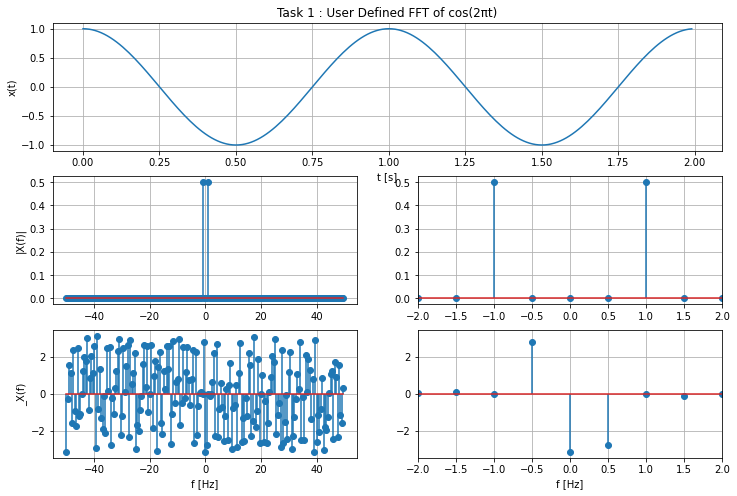
\includegraphics[scale = 0.6]
{txt/Lab9Fig1.png}

Figure 2:

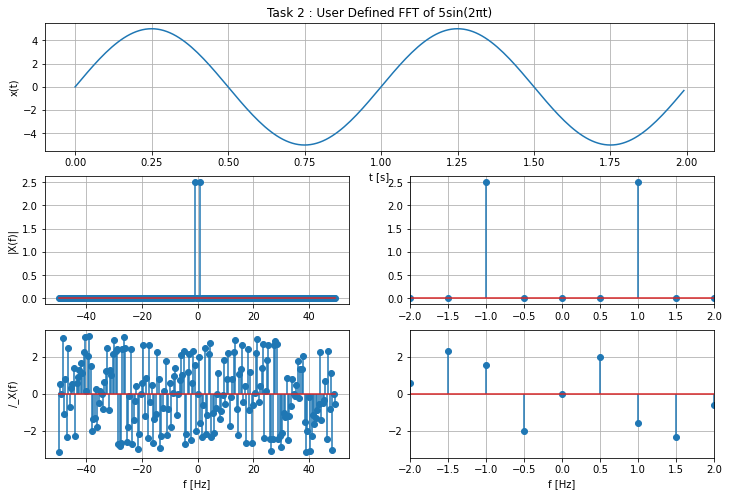
\includegraphics[scale = 0.6]
{txt/Lab9Fig2.png}

Figure 3:

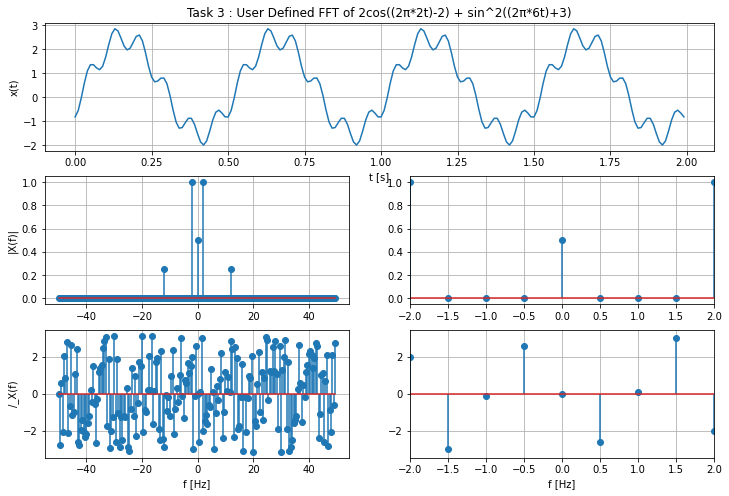
\includegraphics[scale = 0.6]
{txt/Lab9Fig3.png}

Figure 4:

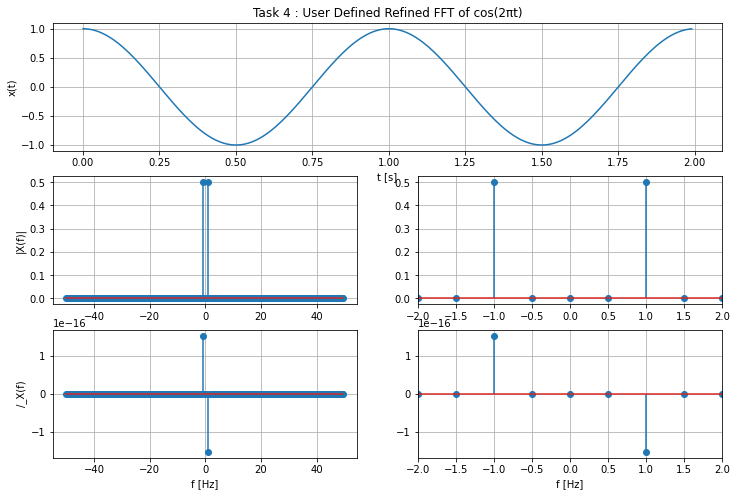
\includegraphics[scale = 0.6]
{txt/Lab9Fig4.png}

Figure 5:

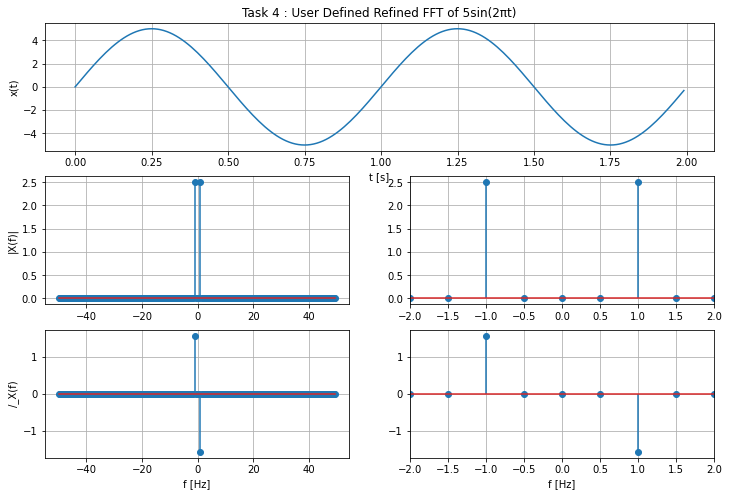
\includegraphics[scale = 0.6]
{txt/Lab9Fig5.png}

Figure 6:

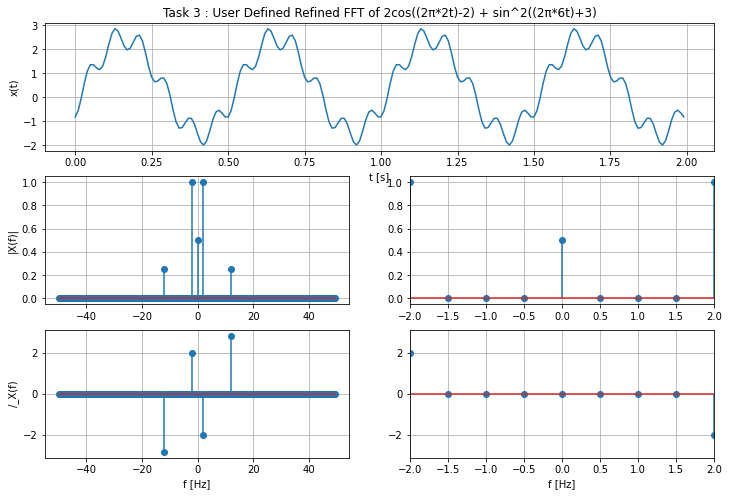
\includegraphics[scale = 0.6]
{txt/Lab9Fig6.png}

Figure 7:

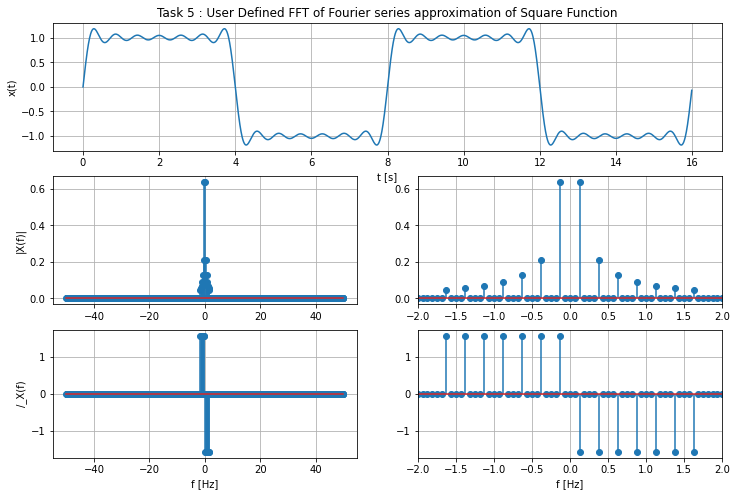
\includegraphics[scale = 0.6]
{txt/Lab9Fig7.png}


\begin{center}
    Conclusion
\end{center}
    This lab helped me gain a better understanding of how to use the fast Fourier transforms in python. This is helpful, because it reduces the need for finding the Fourier series by hand. Also data like magnitudes and phase angles are easy to pull out from the fast Fourier transform function.

\end{document}
%%%%%%%%%%%%%%%%%%%%%%%%%%%%%%%%%%%%%%%%

% Copyright Remarks:
%--------------------

% Copyright holder: Vebjørn S. Førde, copyright: CC BY 4.0
% Note: The author of this template is also the copyright holder.

% Below is an explanation of the CC BY 4.0. Additional statements/ 
% clarifications made by the author/copyright holder are marked with *.

% YOU ARE FREE TO:
% Share — copy and redistribute the material in any medium or format
% Adapt — remix, transform, and build upon the material
% for any purpose, even commercially.

% UNDER THE FOLLOWING TERMS:
% Attribution* — You must give appropriate credit, provide a link to the license,
% and indicate if changes were made. You may do so in any reasonable manner, but 
% not in any way that suggests the licensor endorses you or your use.

% *Note: 
% Attribution NOT NEEDED for: 
%       - PDF distibution (like sharing your PDF document)
%       - Use of (dummy)text and images provided in the template (obviously)
%       - Distributing parts of the template, and not the template as a whole
% I am not really concerned with being given credit. As long as you do not 
% claim to have made the template yourself in distributing it further, I have
% no complaints.

% No additional restrictions — You may not apply legal terms or technological 
% measures that legally restrict others from doing anything the license permits.

% NOTICES:
% No warranties are given.

% Disclaimer* (added by copyright holder):
% THE SOFTWARE IS PROVIDED "AS IS", WITHOUT WARRANTY OF ANY KIND, EXPRESS OR
% IMPLIED, INCLUDING BUT NOT LIMITED TO THE WARRANTIES OF MERCHANTABILITY,
% FITNESS FOR A PARTICULAR PURPOSE AND NONINFRINGEMENT. IN NO EVENT SHALL THE
% AUTHORS OR COPYRIGHT HOLDERS BE LIABLE FOR ANY CLAIM, DAMAGES OR OTHER
% LIABILITY, WHETHER IN AN ACTION OF CONTRACT, TORT OR OTHERWISE, ARISING FROM,
% OUT OF OR IN CONNECTION WITH THE SOFTWARE OR THE USE OR OTHER DEALINGS IN THE
% SOFTWARE.

% Read more about CC BY 4.0:
% https://creativecommons.org/licenses/by/4.0/